\chapter{Jan/24: The dynamic programming problem}
In this course, we are reading
\href{https://web.mit.edu/dimitrib/www/RLCOURSECOMPLETE.pdf}{Bertsekas'
RL book} 11 pages at a time.

The book starts by referring to the recent advances in the RL,
especially AlphaGo and AlphaZero. Even more recent development is the
that DeepMind founder, Demis Hassabis, won 2024 Nobel prize in Chemistry
for his contributions to AlphaFold2, an RL algorithm for predicting
protein folding.

To understand \href{https://www.nature.com/articles/nature16961}{AlphaGo
which came out in 2016}, here's nice clip from
\href{https://www.youtube.com/watch?v=WXuK6gekU1Y&start=2831}{the movie with the
same name}

\hypertarget{two-stages-offline-training-and-online-play}{%
\subsection{Two stages: Offline training and online
play}\label{two-stages-offline-training-and-online-play}}

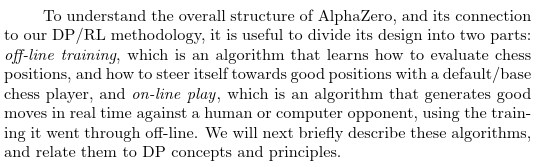
\includegraphics[width=\linewidth]{assets/2025-01-23-offline-online.png}

\hypertarget{policy-network-and-value-network}{%
\subsection{Policy network and value
Network}\label{policy-network-and-value-network}}

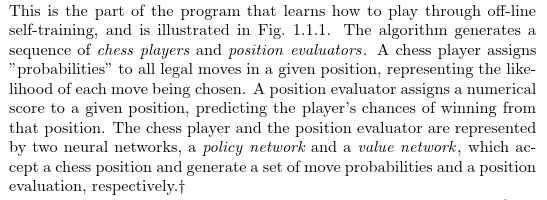
\includegraphics[width=\linewidth]{assets/2025-01-23-two.png}

\hypertarget{policy-evaluation-and-policy-improvement}{%
\subsection{Policy evaluation and policy
improvement}\label{policy-evaluation-and-policy-improvement}}

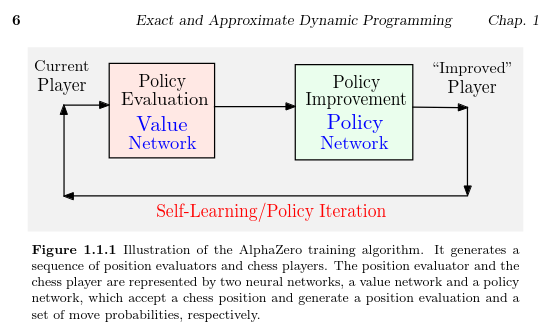
\includegraphics[width=\linewidth]{assets/2025-01-23-fig-1.1.1.png}

\hypertarget{offline-training-and-online-play}{%
\subsection{Offline training and Online
play}\label{offline-training-and-online-play}}

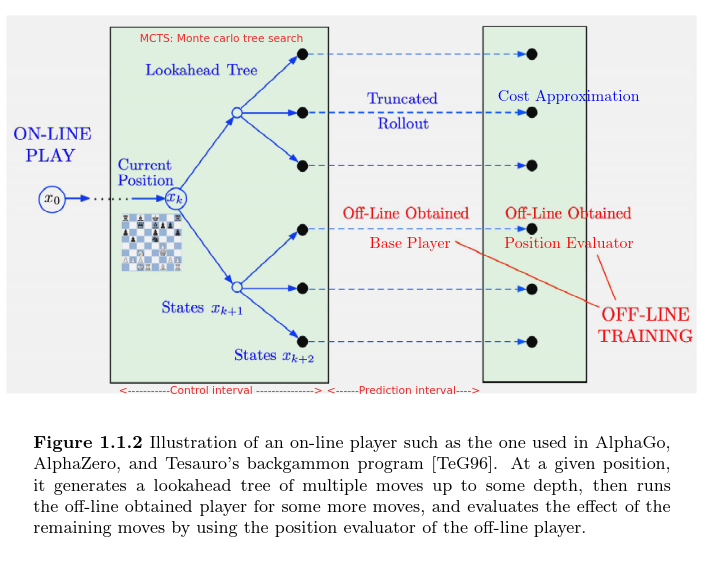
\includegraphics[width=\linewidth]{assets/2025-01-23-fig-1.1.2.png}

\hypertarget{alternative-names-of-rl}{%
\subsection{Alternative names of RL}\label{alternative-names-of-rl}}



Approximations in the value space, also known as \emph{approximate
dynamic programming} or \emph{neuro-dynamic programming}.
\emph{Reinforcement learning} includes both approximations in the value
space and in the policy space. This can be used in control theory as
\emph{model predictive control}.

\hypertarget{finite-horizon-problem-formulation}{%
\subsection{1.2.1 Finite Horizon Problem
Formulation}\label{finite-horizon-problem-formulation}}

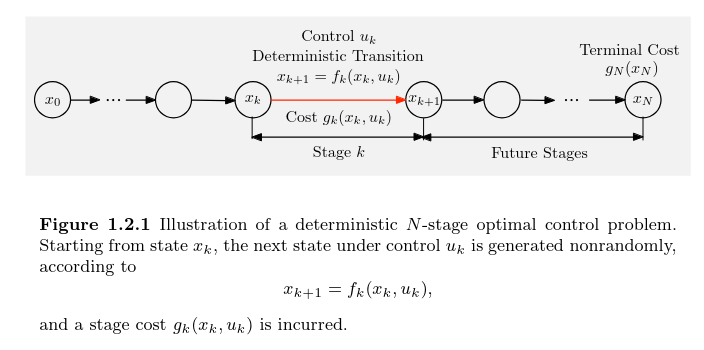
\includegraphics[width=\linewidth]{assets/2025-01-23-fig-1.2.1.png}

The \emph{cost to go} is defined as the summation of step cost
\(g_k(x_k, u_k)\) with a \emph{terminal cost} \(g_N(x_N)\).

\begin{align}
J(x_0; u_0, \dots, u_{N-1}) &= g_N(x_N) + \sum_{k=0}^{N-1} g_k(x_k, u_k), \\
& x_{k+1} &= f_k(x_k, u_k)
\end{align}

We want to minimize the cost over all sequences
\(\{u_0,\dots, u_{N-1}\}\) to find the optimal cost-to-go of \(x_0\),
\begin{align}
J^*(x_0) =  \min_{u_k, k \in \{0, \dots, N-1\}} J(x_0; u_0, \dots, u_{N-1})
\end{align}
